\documentclass[12pt, authoryear]{elsarticle}
\makeatletter
\def\ps@pprintTitle{%
	\let\@oddhead\@empty
	\let\@evenhead\@empty
	\def\@oddfoot{}%
	\let\@evenfoot\@oddfoot}
\makeatother
%\usepackage{lmodern}
% My spacing
\usepackage{setspace}
\setstretch{1.5}
\usepackage{multirow}
%\DeclareMathSizes{12}{14}{10}{10}
\usepackage[margin=2.5cm]{geometry}    % How to set margins - optimized for 2.5cm     
\usepackage{pdfpages} 

% See geometry.pdf to learn the layout options. There are lots.
\geometry{a4paper}                   			% ... or a4paper or a5paper or ... 
\usepackage{enumitem}
\usepackage{mathtools}
%\geometry{landscape}                		% Activate for rotated page geometry
\usepackage[parfill]{parskip}    			% Activate to begin paragraphs with an empty line rather than an indent
\usepackage{graphicx}						% Use pdf, png, jpg, or eps§ with pdflatex; use eps in DVI mode
% TeX will automatically convert eps --> pdf in pdflatex	
\usepackage{flafter}			
\usepackage{setspace}
%\linespread{1.5}
\usepackage[font={}]{caption}
\usepackage[bottom]{footmisc}
\usepackage[capposition=top]{floatrow}   %figure notes
\usepackage{lscape}
\usepackage[toc,page]{appendix}
%math packages 
\usepackage{amssymb}
\usepackage{fancyhdr}
\usepackage{graphicx,epsf,subfigure}
\usepackage{pstricks,pst-node,psfrag}
\usepackage{amsthm,amssymb,amsmath}
\usepackage{amsmath,bm}
\graphicspath{ {plots/} }

%mathnotes
\newcommand{\bbeta}{\mbox{\boldmath $\beta$}}
\newcommand{\beps}{\mbox{\boldmath $\epsilon$}}
\newcommand{\bX}{\mbox{\boldmath $X$}}
\newcommand{\bY}{\mbox{\boldmath $Y$}}
\newcommand{\bI}{\mbox{\boldmath $I$}}
\newcommand{\N}{\mathcal{N}}
\newcommand{\x}{\textsc{\textbf{x}}}
\newcommand{\xx}{\textsc{x}}
\definecolor{aurometalsaurus}{rgb}{0.43, 0.5, 0.5}
%add figure 
\DeclareGraphicsRule{.tif}{png}{.png}{`convert #1 `dirname #1`/`basename #1 .tif`.png}
\usepackage{rotating}
\usepackage{pdflscape}
\usepackage{hyperref}
\usepackage[round]{natbib}
	\definecolor{ashgrey}{rgb}{0.7, 0.75, 0.71}
\usepackage{soul}

\def\bibsection{\section{References}} %%% Make "References" appear before bibliography
\usepackage{longtable}
\usepackage{hyperref}
\usepackage{tablefootnote}
\usepackage{lscape} 
\usepackage{animate}
\usepackage{algorithm}
\usepackage[noend]{algpseudocode}

\renewcommand{\contentsname}{Table of Contents} % change name from Contents to Table of Contents

\usepackage{titlesec}

\setcounter{secnumdepth}{4}

%_______________________________________________________________________________________________________%
%_______________________________________________________________________________________________________%
%\usepackage[table]{xcolor}% http://ctan.org/pkg/xcolor
%\usepackage{graphicx,multirow}
\usepackage{xcolor,colortbl}
\usepackage{xcolor}
%\usepackage{graphicx,multirow}
\usepackage[capposition=top]{floatrow}
\setcounter{secnumdepth}{4}
\usepackage{tikz}
\begin{document}

\begin{frontmatter}  %

\title{Who's hot and who's not? \\  Uncovering consistency in NBA players using Hidden Markov Models}

\author[Add1]{Felix Adam}
\ead{felix.adam@barcelonagse.eu}

\author[Add1]{Julia Barnett}
\ead{julia.barnett@barcelonagse.eu}

\author[Add1]{Oscar Mart\'inez}
\ead{oscar.martinez@barcelonagse.eu}

\author[Add1]{Guillem Sitges}
\ead{guillem.sitges@barcelonagse.eu}

\address[Add1]{Barcelona Graduate School of Economics, Barcelona, Spain}


%\begin{abstract}
%\small{
%Abstract to be written here. 
%}
%\end{abstract}

%\vspace{1cm}

\begin{keyword}
\footnotesize{
Hidden Markov Models  \sep Sports Analytics \sep  Dynamic Programming \\ \vspace{0.3cm}
%\textit{JEL classification} L250 \sep L100
}
\end{keyword}
\vspace{0.5cm}
\end{frontmatter}

\headsep 35pt % So that header does not go over title
\begin{abstract}
This project aims to investigate...
\end{abstract}

\section{Introduction}

The hot hand fallacy  is a well known issue in sports analytics and human perception. First discussed by \cite{gilovich1985hot}, it describes the misconception that players tend to have higher chances of scoring points if they have scored in the previous shot. However, a look at sports media reveals that the concept of being ``hot" is still in use today. We try to approach the concept of ``hotness" from a different angle; we look at overall game performance rather than single outcomes such as shots made. We assume that a player's performance in each NBA game in fact depends on an underlying hidden state such as ``hot" or ``cold". Using game-level data for the 2017-18 and 2018-19 NBA seasons, we fit a Hidden Markov Model to uncover these states. Our results closely align with common conceptions about current players in the NBA. Superstars such as James Harden and Lebron James tend to stay ``hot", and even when ``cold" they have above-average games. The average player, however, tends to only have an average game when he is hot. While our results should not be interpreted as a proof for ``hotness", they can be used as a tool for scouting reports or management decisions because they jointly describe a player's performance and consistency. 

\section{Data and Features}

Our analysis is based on player-level data for each game in the 2017-18 and 2018-19 NBA seasons. We have obtained the data from www.basketball-reference.com using web-scraping methods. The data of interest to us was specifically taken from the game logs of players during the 2017-18 season and the 2018-19 season. There are 82 games in a season, so with data on 497 players we have a total of 26,003 observations in the first data set (2017-18 season) and 387 players and 20,228 observations in the second data set (2018-2019 season, which has yet to finish).The data included information for every player and each game played; some statistics reported include seconds played, shot percentages, rebounds, assists, steals, blocks, turnovers, points, the overall game score, and their plus minus score. Overall distributions for these statistics can be found in \ref{overall_dist}.

Instead of focusing on a single outcome measure, we created a ``Game Value Index" ($GV$) using a combination of these statistics. This simplified the analysis given that the different statistics have different distributions. Further, it can be used to obtain an overall view of a player's impact in a game. The metric is derived by combining the most important positive individual statistics (field goal percentage, three-point percentage, free throw percentage, total rebounds, steals, assists, blocks, and total points), subtracting the negative one (turnovers), and finally dividing by the seconds played per game to standardize the metric per game (see \ref{game_value_dist} for overall distributions).

\begin{align*}
GV = \frac{\text{\%FG + \%3PT + \%FT + Rebound + Steal + Assist +  Block + Points - Turnovers}}{\text{Seconds Played}}
\end{align*} 

To further simplify the analysis, we created a discrete variable called ``Game Quality" from the Game Value Index. A player had a good game if his Game Value Index was above the $70^{th}$ percentile of all games, a bad game if his outcome was below the $30^{th}$ percentile and an average game between these two. We then used this Game Quality measure as our observation in the context of a Hidden Markov Model.

\section{Analysis}

\subsection{Model}

As described, we assumed that a player's performance can be described by a Hidden Markov Model with the following structure:

\begin{center}

\tikzset{every picture/.style={line width=0.75pt}} %set default line width to 0.75pt        

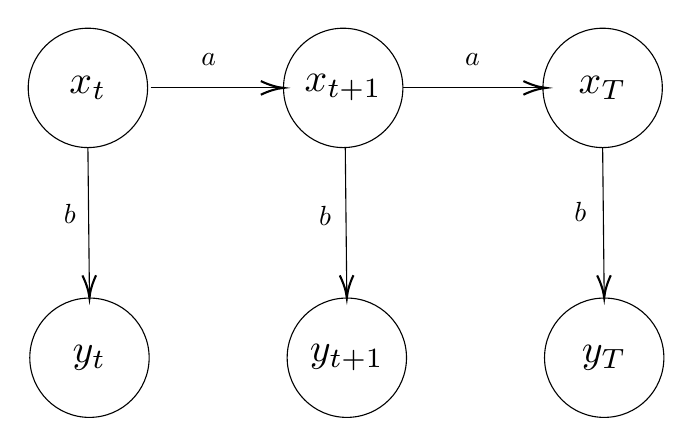
\begin{tikzpicture}[x=0.75pt,y=0.75pt,yscale=-1,xscale=1]
%uncomment if require: \path (0,419); %set diagram left start at 0, and has height of 419

%Shape: Circle [id:dp5666590298051767] 
\draw   (166,85.75) .. controls (166,69.87) and (178.87,57) .. (194.75,57) .. controls (210.63,57) and (223.5,69.87) .. (223.5,85.75) .. controls (223.5,101.63) and (210.63,114.5) .. (194.75,114.5) .. controls (178.87,114.5) and (166,101.63) .. (166,85.75) -- cycle ;
%Shape: Circle [id:dp055618042838002535] 
\draw   (289,85.75) .. controls (289,69.87) and (301.87,57) .. (317.75,57) .. controls (333.63,57) and (346.5,69.87) .. (346.5,85.75) .. controls (346.5,101.63) and (333.63,114.5) .. (317.75,114.5) .. controls (301.87,114.5) and (289,101.63) .. (289,85.75) -- cycle ;

%Shape: Circle [id:dp721119784913766] 
\draw   (414,85.75) .. controls (414,69.87) and (426.87,57) .. (442.75,57) .. controls (458.63,57) and (471.5,69.87) .. (471.5,85.75) .. controls (471.5,101.63) and (458.63,114.5) .. (442.75,114.5) .. controls (426.87,114.5) and (414,101.63) .. (414,85.75) -- cycle ;

%Straight Lines [id:da33403214567957407] 
\draw    (225,85.75) -- (287,85.75) ;
\draw [shift={(289,85.75)}, rotate = 180] [color={rgb, 255:red, 0; green, 0; blue, 0 }  ][line width=0.75]    (10.93,-3.29) .. controls (6.95,-1.4) and (3.31,-0.3) .. (0,0) .. controls (3.31,0.3) and (6.95,1.4) .. (10.93,3.29)   ;

%Straight Lines [id:da43789227763392435] 
\draw    (346.5,85.75) -- (413.5,85.75) ;
\draw [shift={(415.5,85.75)}, rotate = 180] [color={rgb, 255:red, 0; green, 0; blue, 0 }  ][line width=0.75]    (10.93,-3.29) .. controls (6.95,-1.4) and (3.31,-0.3) .. (0,0) .. controls (3.31,0.3) and (6.95,1.4) .. (10.93,3.29)   ;

%Straight Lines [id:da8759139427531057] 
\draw    (194.75,114.5) -- (195.48,185) ;
\draw [shift={(195.5,187)}, rotate = 269.40999999999997] [color={rgb, 255:red, 0; green, 0; blue, 0 }  ][line width=0.75]    (10.93,-3.29) .. controls (6.95,-1.4) and (3.31,-0.3) .. (0,0) .. controls (3.31,0.3) and (6.95,1.4) .. (10.93,3.29)   ;

%Shape: Circle [id:dp3016810713511464] 
\draw   (166.75,215.75) .. controls (166.75,199.87) and (179.62,187) .. (195.5,187) .. controls (211.38,187) and (224.25,199.87) .. (224.25,215.75) .. controls (224.25,231.63) and (211.38,244.5) .. (195.5,244.5) .. controls (179.62,244.5) and (166.75,231.63) .. (166.75,215.75) -- cycle ;

%Straight Lines [id:da4575372266521941] 
\draw    (318.75,114.5) -- (319.48,185) ;
\draw [shift={(319.5,187)}, rotate = 269.40999999999997] [color={rgb, 255:red, 0; green, 0; blue, 0 }  ][line width=0.75]    (10.93,-3.29) .. controls (6.95,-1.4) and (3.31,-0.3) .. (0,0) .. controls (3.31,0.3) and (6.95,1.4) .. (10.93,3.29)   ;

%Shape: Circle [id:dp7524853971441587] 
\draw   (290.75,215.75) .. controls (290.75,199.87) and (303.62,187) .. (319.5,187) .. controls (335.38,187) and (348.25,199.87) .. (348.25,215.75) .. controls (348.25,231.63) and (335.38,244.5) .. (319.5,244.5) .. controls (303.62,244.5) and (290.75,231.63) .. (290.75,215.75) -- cycle ;
%Straight Lines [id:da3534338299500158] 
\draw    (442.75,114.5) -- (443.48,185) ;
\draw [shift={(443.5,187)}, rotate = 269.40999999999997] [color={rgb, 255:red, 0; green, 0; blue, 0 }  ][line width=0.75]    (10.93,-3.29) .. controls (6.95,-1.4) and (3.31,-0.3) .. (0,0) .. controls (3.31,0.3) and (6.95,1.4) .. (10.93,3.29)   ;

%Shape: Circle [id:dp09641139918136554] 
\draw   (414.75,215.75) .. controls (414.75,199.87) and (427.62,187) .. (443.5,187) .. controls (459.38,187) and (472.25,199.87) .. (472.25,215.75) .. controls (472.25,231.63) and (459.38,244.5) .. (443.5,244.5) .. controls (427.62,244.5) and (414.75,231.63) .. (414.75,215.75) -- cycle ;


% Text Node
\draw (194.75,85.75) node [scale=1.44]  {$x_{t}$};
% Text Node
\draw (317.75,85.75) node [scale=1.44]  {$x_{t+1}$};
% Text Node
\draw (442.75,85.75) node [scale=1.44]  {$x_{T}$};
% Text Node
\draw (195.5,215.75) node [scale=1.44]  {$y_{t}$};
% Text Node
\draw (319.5,215.75) node [scale=1.44]  {$y_{t+1}$};
% Text Node
\draw (443.5,215.75) node [scale=1.44]  {$y_{T}$};
% Text Node
\draw (253,72.25) node   {$a$};
% Text Node
\draw (380,72.25) node   {$a$};
% Text Node
\draw (186,146.25) node   {$b$};
% Text Node
\draw (309,147.25) node   {$b$};
% Text Node
\draw (432,145.25) node   {$b$};

\end{tikzpicture}

\end{center}

In which we only observe the outcomes $y_t$. The primitives are defined as follows:

\begin{itemize}
	\item $x_t \in [\text{Cold, Hot}]$, the hidden state
	\item $y_t \in [\text{Bad, Average, Good}]$, the observed outcomes as described in the previous section
	\item $b_{ij} = P(Y = j | X = i)$, the emission probabilities of observing a game outcome conditioned on being hot or cold
	\item $a_{ij} = P(X_{t+1} = j | X_t =i)$, the transition probabilities of changing from a given state to another (or staying at the same state) between periods
	\item $\pi_i$: the initial probabilities of transitioning to a hidden state (priors)
\end{itemize}

The most important model assumption is that the state $x_t$ only depends on the previous state $x_{t-1}$ and is conditionally independent of all other previous states. In the basketball context, this means that the probability of being hot or cold in the current game only depends on the previous game. We acknowledge that this is quite a strong assumption, particularly given the research on the hot hand fallacy. However, even though we cannot assume any predictive power of our model, we argue that it helps to uncover overall player quality. This is further supported by the consistency of our results over the two observed seasons as shown in section \ref{results}.

\subsubsection{Fitting the Model}

Our main interest lies in the transition and emission probabilities for each player as a measure of consistency and overall performance. We use the Baum-Welch algorithm to uncover these as the parameters of the Hidden Markov Model. The algorithm makes use of dynamic programming and an Expectation-Maximization procedure to fit the model to a given data set. We follow \cite{rabiner1989tutorial} for the derivation of the algorithm.

The parameters to be estimated are those of the HMM: 
\begin{itemize}
	\item \textbf{Transition matrix}: denoted by $A=\left\{a_{i j}\right\}=P\left(X_{t}=j | X_{t-1}=i\right)$
	\item \textbf{Emission matrix}: denoted by $b_{j}\left(y_{i}\right)=P\left(Y_{t}=y_{i} | X_{t}=j\right)$ and $B$ the collection of $b_{j}$. Generally, a distribution is assumed and this matrix contains the different parameters for each state of the assumed distribution
	\item \textbf{Initial parameters/Priors}: denoted by $\pi_{i}=P\left(X_{1}=i\right)$
\end{itemize}

Given a sequence of observations $Y = {y_{1},...,y_{T}}$, the algorithm will find the parameters $ A, B$ and $\pi$ that maximize the probability of the observed sequence. We will now describe the algorithm in detail, following the steps described by \cite{rabiner1989tutorial}.

\subsubsection{Forward step}

In the forward step we compute the probability of observing the sequence $Y$ and being in a state $x$ at time $t$, given the parameters $\theta$ as $\alpha_{i}(t)=P\left(Y_{1}=y_{1}, \ldots, Y_{t}=y_{t}, X_{t}=i |\theta \right)$. This step is computed from the first period to the last. It is initialized in period one using the priors and the emission probabilities $b$:

$$  \alpha_{i}(1)=\pi_{i} b_{i}\left(y_{1}\right) $$

The subsequent steps are computed as:
$$  \alpha_{i}(t+1)=b_{i}\left(y_{t+1}\right) \sum_{j=1}^{S} \alpha_{j}(t) a_{j i} $$

\subsubsection{Backward Step}

In the backward step, the probabilities of observing the remaining sequence given an assumed state $x$ in time $t$ are computed as $\beta_{i}(t)=P\left(Y_{t+1}=y_{t+1}, \ldots, Y_{T}=y_{T} | X_{t}=i, params\right)$. This step is computed from the last period to the first. The last period is initialized as $\beta_{i}(T)=1$.

Then, using induction, each previous step will be computed as: 
$$ 
\beta_{i}(t)=\sum_{j=1}^{S} \beta_{j}(t+1) a_{i j} b_{j}\left(y_{t+1}\right)
$$

Both the backward and forward step make use of dynamic programming by storing previous results for subsequent calculations. Using the forward and backward step, we do not need to compute all possible probabilities for all sequences at each step which dramatically reduces computational complexity.

\subsubsection{Updates}
Once the Forward and Backward step are computed, we can proceed to compute the temporary variables $\gamma$ and $\xi$ that will be used to update the parameters. This is the estimation step.

$\gamma_i(t)$ describes the probability of being in state $i$ at time $t$ given the sequence $Y$ and the current parameters $\theta$. 
 $$ 
 \gamma_{i}(t)=P\left(X_{t}=i | Y, \theta\right)=\frac{P\left(X_{t}=i, Y | \theta \right)}{P(Y | \theta)}=\frac{\alpha_{i}(t) \beta_{i}(t)}{\sum_{j=1}^{N} \alpha_{j}(t) \beta_{j}(t)}
 $$
 
$\xi$ is used to compute the probability of transitioning from a state $i$ to another state $j$ at a given point in time. It computes the joint probability of observing the sequence and a defined transition, and also normalizes it by the probability of observing the sequence.
 
\begin{align*}
 \xi_{i j}(t) =P\left(X_{t}=i, X_{t+1}=j | Y, \theta \right) &=\frac{P\left(X_{t}=i, X_{t+1}=j, Y | \theta\right)}{P(Y | \theta)} \\
 &=\frac{\alpha_{i}(t) a_{i j} \beta_{j}(t+1) b_{j}\left(y_{t+1}\right)}{\sum_{i=1}^{N} \sum_{j=1}^{N} \alpha_{i}(t) a_{i j} \beta_{j}(t+1) b_{j}\left(y_{t+1}\right)}
\end{align*} 
 
Having calculated $\gamma$ and $\xi$, we can update $\theta = (A,B,\pi)$ in the maximization step.

\begin{itemize}
 	\item Transition matrix: $$ 
 	a_{i j}^{*}=\frac{\sum_{t=1}^{T-1} \xi_{i j}(t)}{\sum_{t=1}^{T-1} \gamma_{i}(t)}
 	$$
 	
 	\item Emission matrix: 
 	
 	$$ 
 	b_{i}^{*}\left(v_{k}\right)=\frac{\sum_{t=1}^{T} 1_{y_{t}=v_{k}} \gamma_{i}(t)}{\sum_{t=1}^{T} \gamma_{i}(t)}
 	$$
 	
 	\item Priors: given by the first parameter of the $\gamma$ sequence $\pi_{i}=\gamma_{i}(1)$
\end{itemize}

These steps are repeated iteratively. In our case we have used a fixed number of iterations. Generally, the algorithm is guaranteed to find a better set of parameters $\theta$ at each step $k$. It is guaranteed that at each step $P(Y|\theta_{k+1})>P(Y|\theta_{k})$. However, the algorithm might converge to a local maximum, so it is best practice to initialize the algorithm with new starting parameters and repeat the estimation (\cite{rabiner1989tutorial}). Then, the results can be averaged to obtain the final parameters. The implementation of the algorithm can be found in \ref{algo}

\newpage

\section{Results}\label{results}

We run the algorithm for each player and season to obtain the emission and transition parameters. For each player, we use the same priors to initialize the algorithm. The maximum number of iterations is set to 50.  First, we present the overall parameter distributions.

\subsection{Transmission and Emission Probabilities}

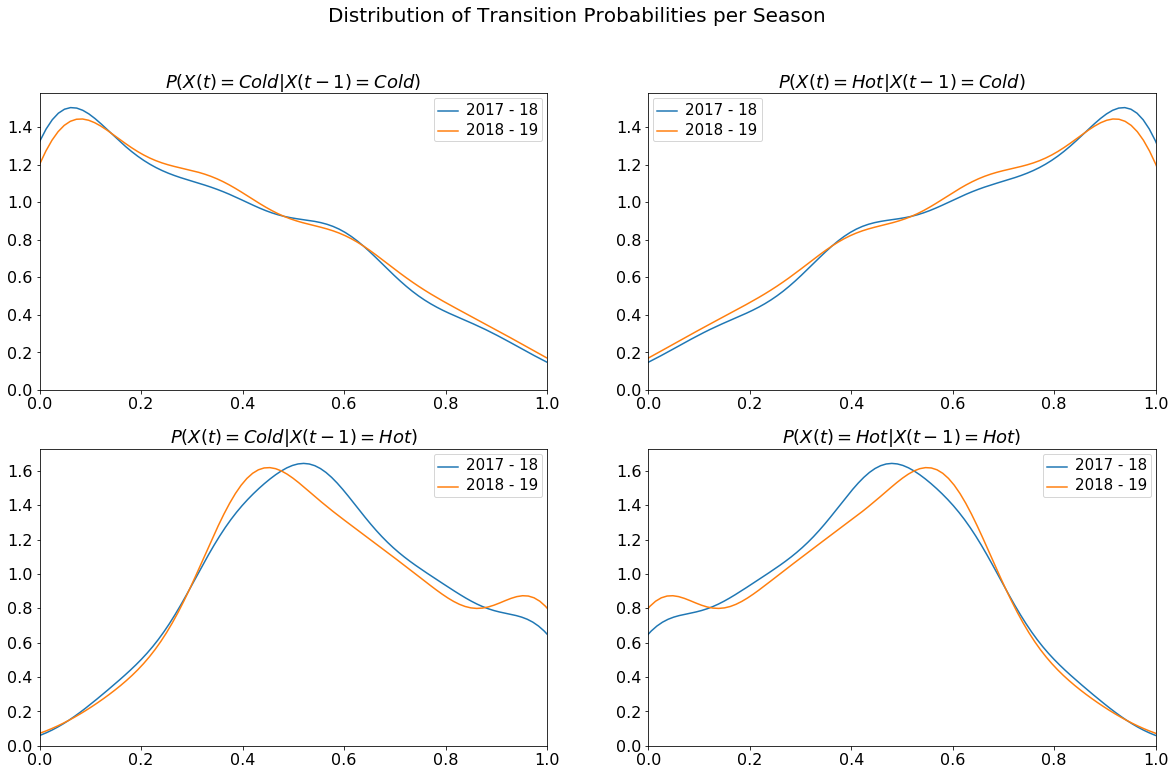
\includegraphics[scale=0.4]{2distoftransition_probs_perseason}

First we note that the distributions are complements, which is given due to the fact that we only included the two hidden states. Looking at the top row, we see that it is actually quite unlikely for players to stay cold. As shown in the top right plot, most players have a high probability of transitioning from cold to hot. However, we also see that not many players have a high probability of staying hot, as shown in the bottom right plot. This makes sense given the many players in the NBA yet the select few that are identified as “superstars”. These consistent players are on the right tail of the Hot$\rightarrow$Hot plot (bottom right); this zone of outstanding players seems to be even rarer than the “awful” players who seem to fall in the Cold$\rightarrow$Cold zone for a large proportion of the time. A key takeaway is that what makes a good player is the high probability of staying in this hot zone, not just the ability to recover from a cold game.

Obviously, the transition probabilities alone are not conclusive; it is important that when the player is hot, he also has a good game. In order to better understand this we need to also analyze the emission data. 

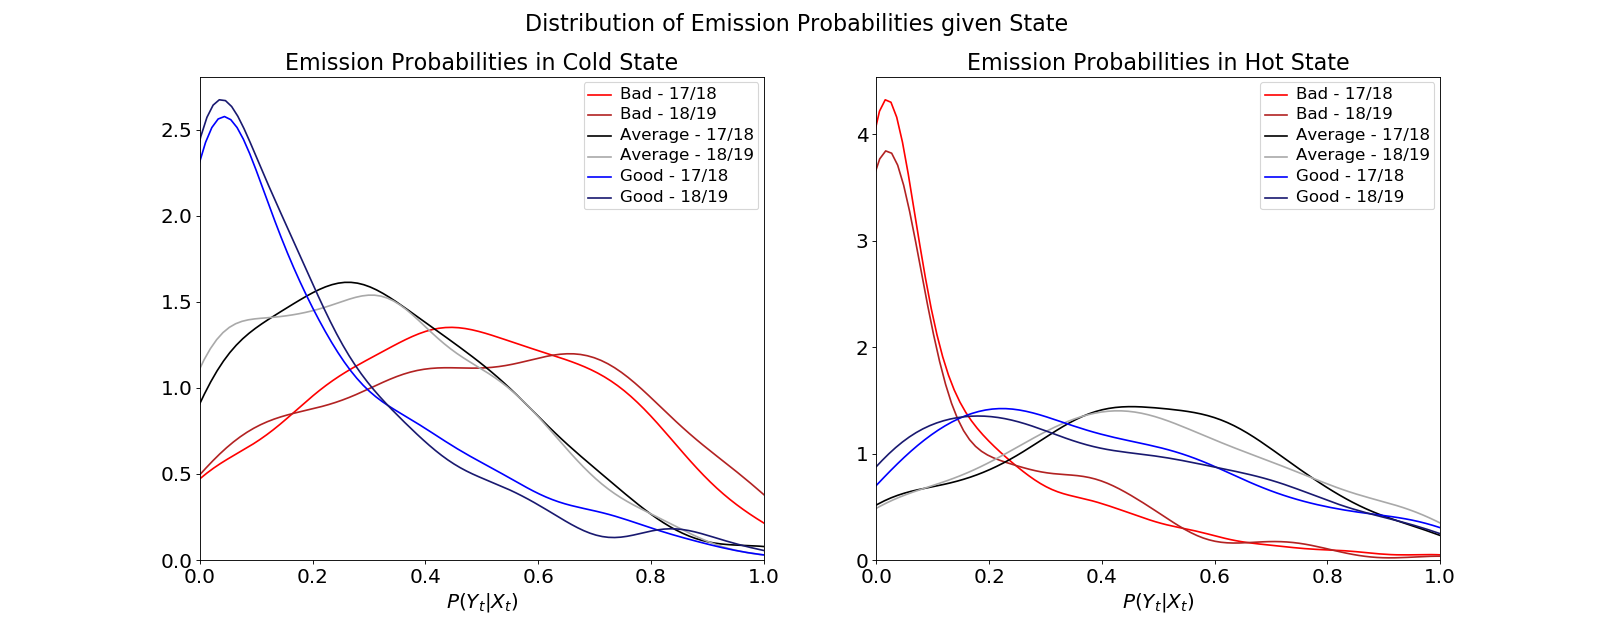
\includegraphics[scale=0.35]{emission_probs}

We can see that for most players in the cold zone, it is almost impossible to have a good game (blue lines), and having a bad game is the most likely event although some players have average games while cold. Contrarily, when a player is hot, it is unlikely they will have a bad game. Interestingly, the emission probabilities of having an average game when hot are on average higher than the probability of having a good game. We can therefore conclude that average players tend to have average games when hot. This leads us to the observation that superstars are the players who almost certainly perform good while hot, and still perform average or even good while cold.

For both emission and transition probabilities, we see almost no changes in distribution. This supports the underlying model assumptions. If the model would just fit noise, we'd expect the distributions to differ over seasons. 

\subsection{Top Players}

We now use our results to identify the top performers of the 2017-18 season. These are players that have a low probability of staying cold, a high probability of staying hot, a high probability of having a great game even while cold, and even further are almost certain to have a good game while hot. The results are summarized in \ref{top_players}.

The majority of these players seem very intuitively correctly identified; our algorithm consistently identifies the superstars of the NBA. These are the players who rarely have a bad game and stay hot with much higher probabilities than average. Interestingly, even these superstars stay in the hot zone with a probability less than 0.65, so this might not be a defining characteristic of a good player. Instead, what seems more important is that even if the player is not in a hot zone, they are still outperforming the other players (who could very well be hot). Additionally, once these players are hot they are certain to dominate the court; even when they are cold, Lebron, Davis, Embiid, and Harden will have a good game with probability greater than 0.8.
 
Further we can look into changes between the two seasons: players who dropped out or are rising stars in 2018-19 (see \ref{top_players}). Unsurprisingly, Giannis is a rising star during this season. Cousins and Whiteside fell out of the leaderboard, but the rest of our stars maintained their positions with dignity.

The consistency of our results on a player basis further supports the use of a HMM.

\subsection{Bad Players}

Finally, we can look at the apologetically dreadful players (\ref{bad_players}). These guys are the ones who almost always stay cold, when they are cold will certainly have a bad game, and even when hot will only have an average game. Interestingly, they only ever seem to have average games. However, these are still NBA players and are certainly earning salaries that help them get through seeing their name on this pitiful list (for reference, Wesley Johnson is projected to earn \$6,134,000 during this season). 

\section{Discussion}

\subsection{Extensions}

Ultimately, even though our model results seem to be consistent over seasons, the next step would be to perform model diagnostics such as testing for Markov properties. Further,  our analysis relies on the use of the discrete Game Quality observation. Subsequent analyses could use different outcome measures to describe the joint distributions of statistics such as shots made and assists. 

\subsection{Potential Use Cases}

The GameValueIndex itself could be modified to fit the goals of the end user. For example, if a coach wanted to sign a good defensive player then they could assign greater weights to rebounds, blocks, steals, etc. Likewise, the analysis could be used to select the Most Valuable Player of Defensive Player of the Year. From a management perspective you could also filter for players with low contracts in order to find highly consistent players that are extremely valuable for their cost. Most improved players are easy to identify; a player that becomes more consistently good is much more desirable than a streaky player. Coaches could also use this information for load-management for players. They could build optimal player rotations which ensure that at least one or two consistent players are playing in each game. 

\section{Conclusion}

We have fit a Hidden Markov Model on player level data for the NBA seasons 2017-18 and 2018-19 to uncover player quality and consistency. We have assumed that players can be either hot or cold and perform accordingly. Our results are closely aligned with the common perception of players, such as superstars like Harden and James. Very good players tend to have average or even good games when hot and are unlikely to stay cold. Average players tend to have only average games, even when hot. Our anlaysis can be used for scouting reports or team-management decisions. 



%_______________________________________________________________________________________________________%
%BIBLIOGRAPHY
%_______________________________________________________________________________________________________%
\pagebreak
\bibliographystyle{agsm}
\setcitestyle{authoryear}
\bibliography{SMO.bib}

\appendix

\section{Overall Distributions} \label{overall_dist}

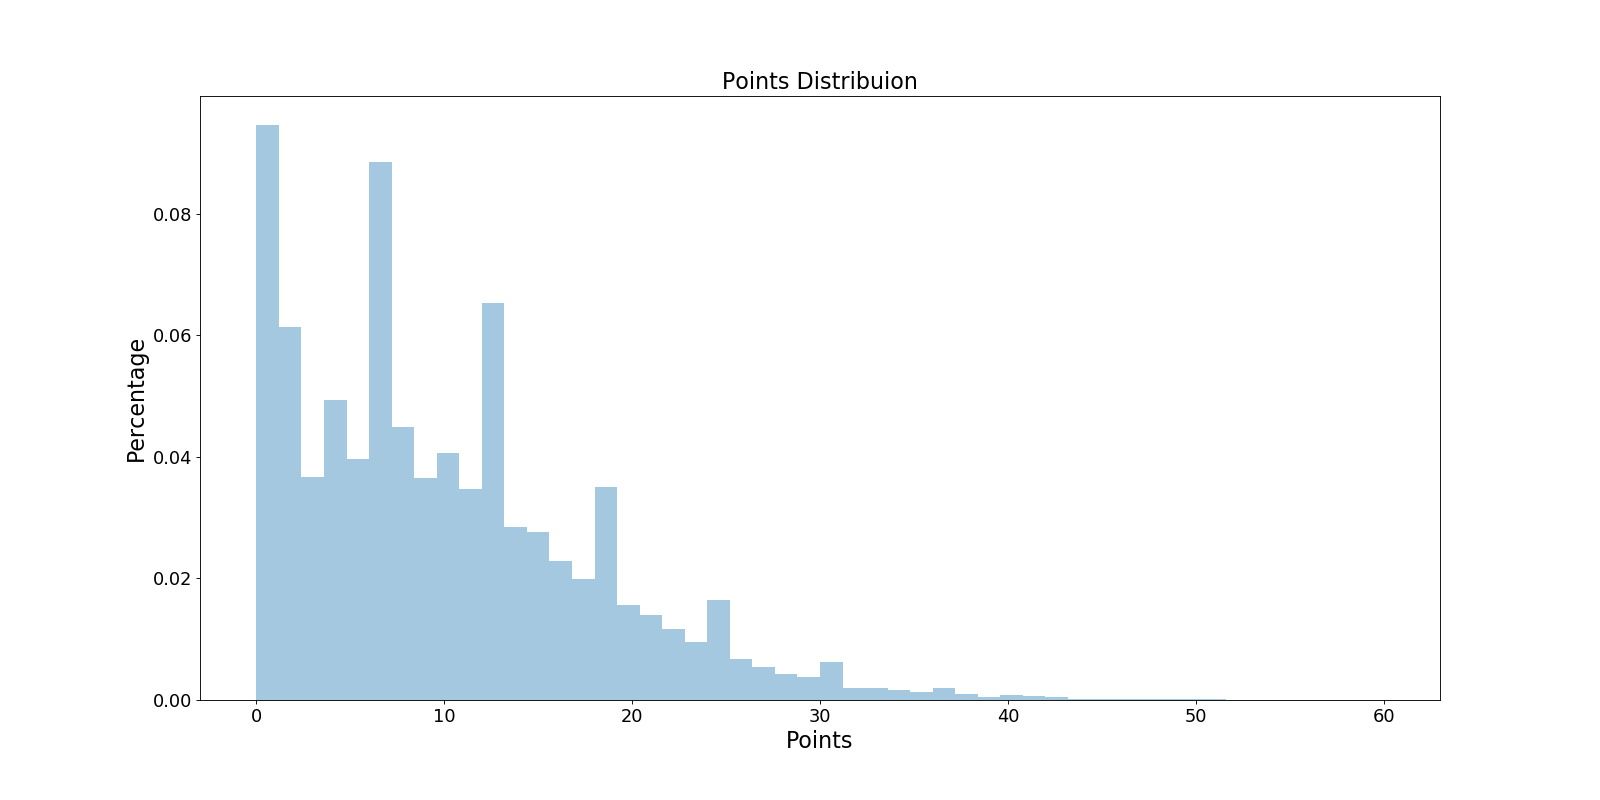
\includegraphics[scale=0.3]{Points_Distribution}\\
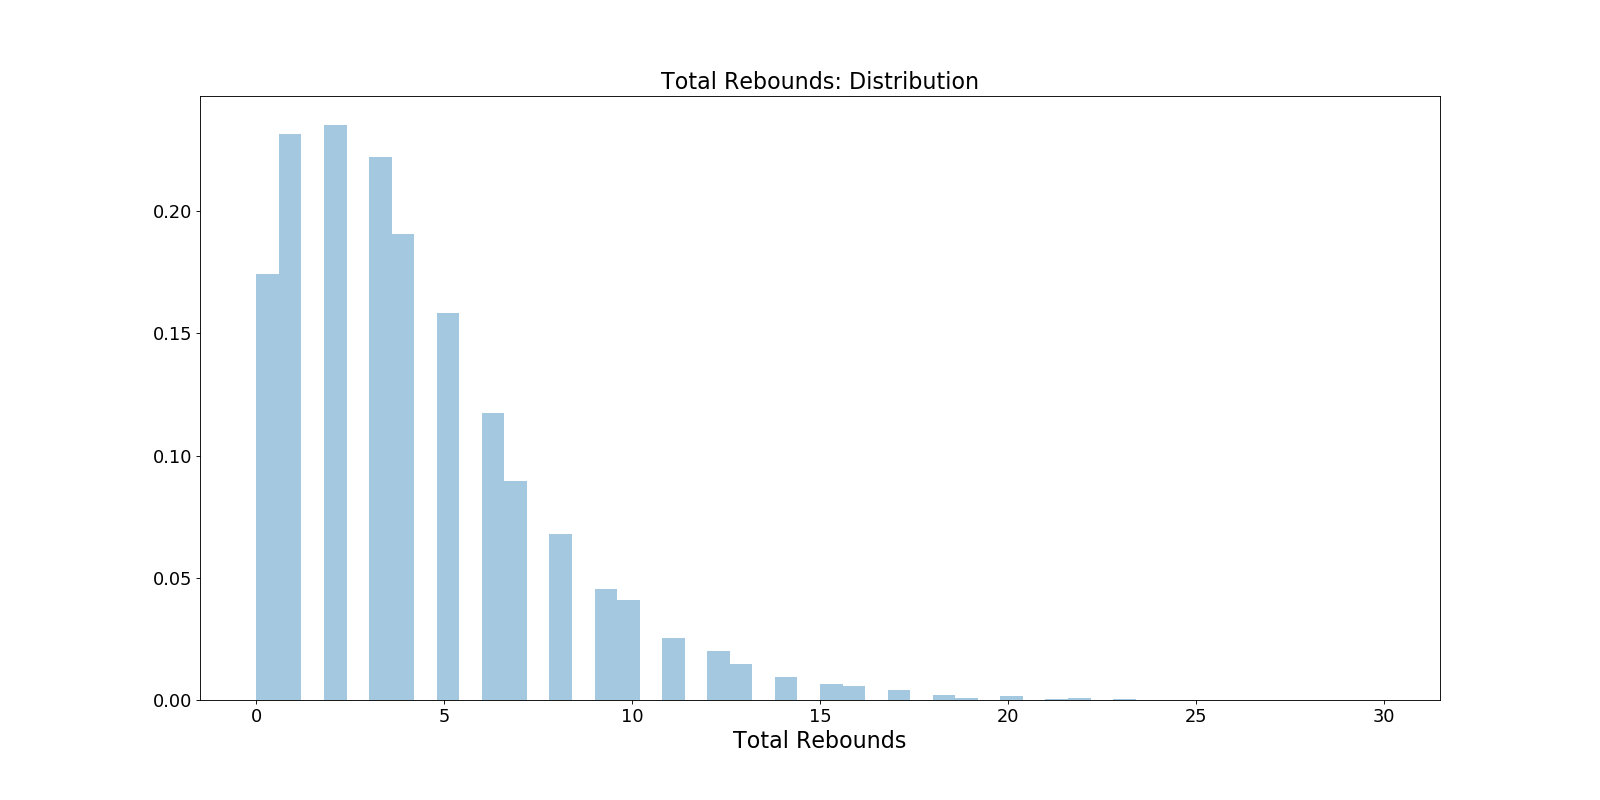
\includegraphics[scale=0.3]{Rebounds_Distribution}\\
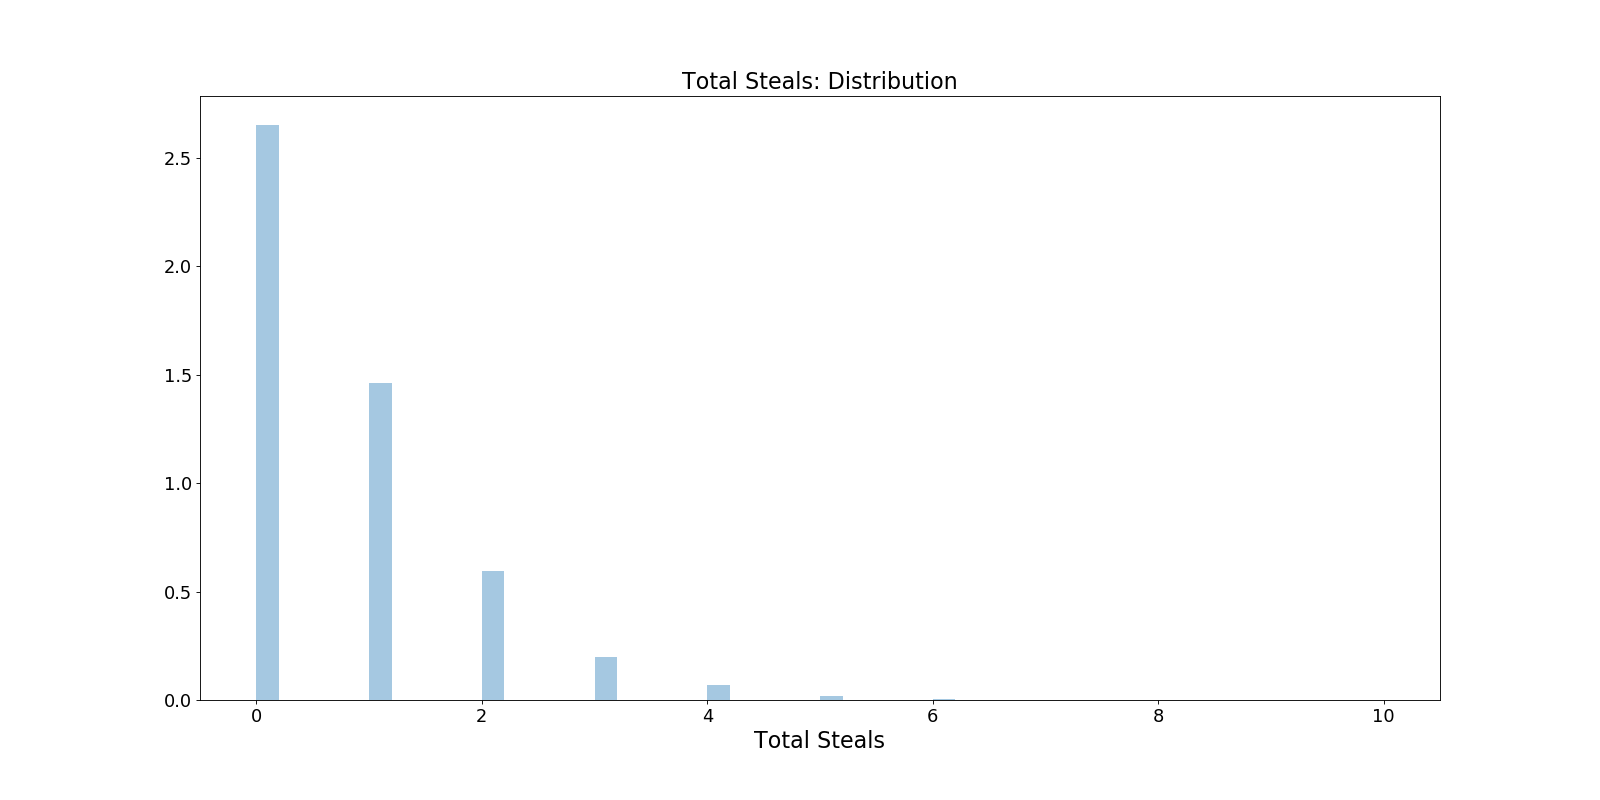
\includegraphics[scale=0.3]{Steals_Distribution}\\
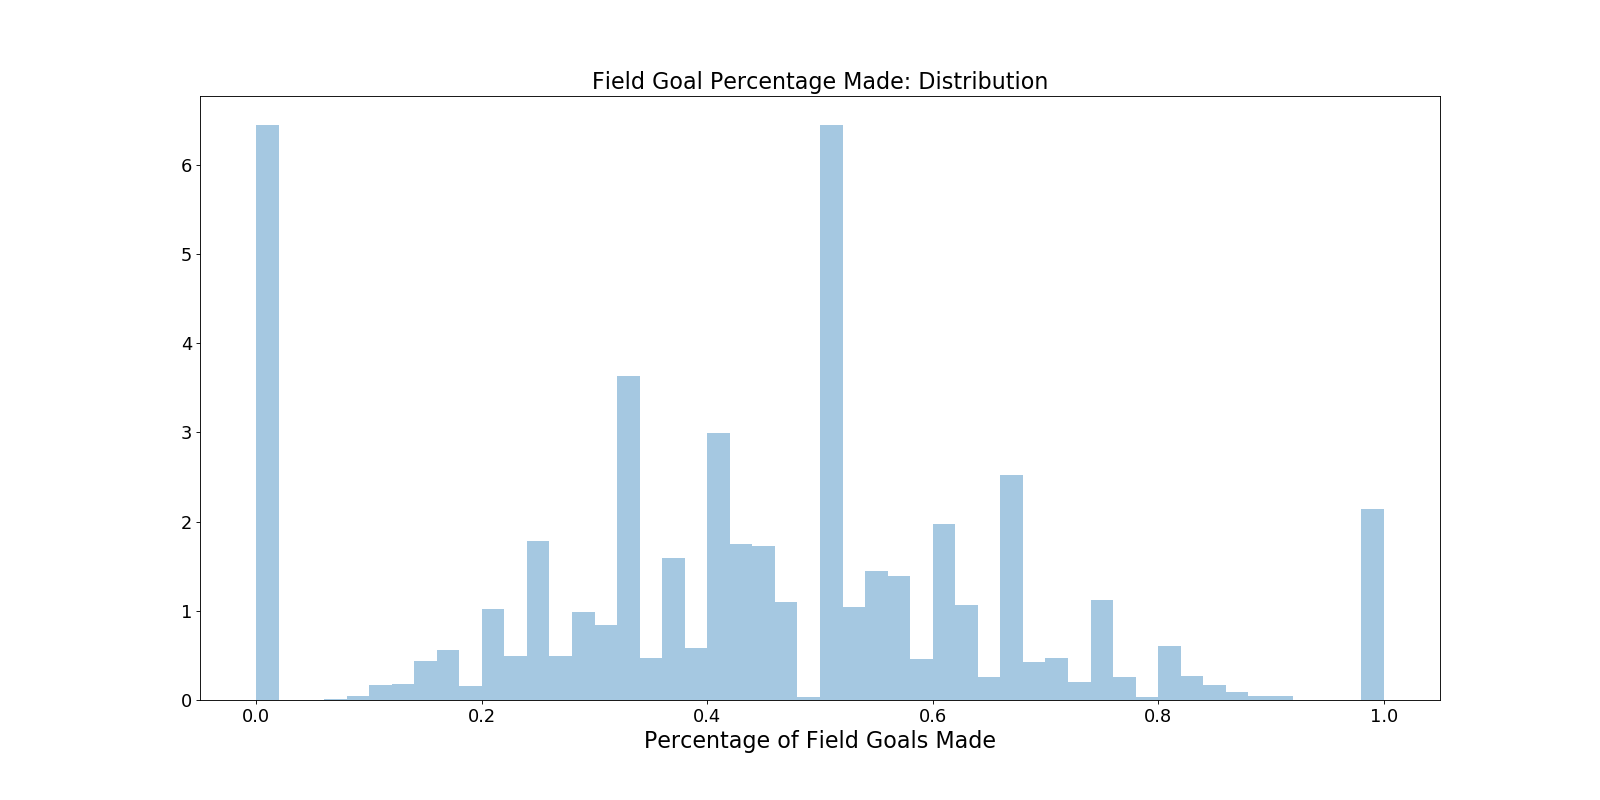
\includegraphics[scale=0.3]{FG_Percent_Distribution}\\
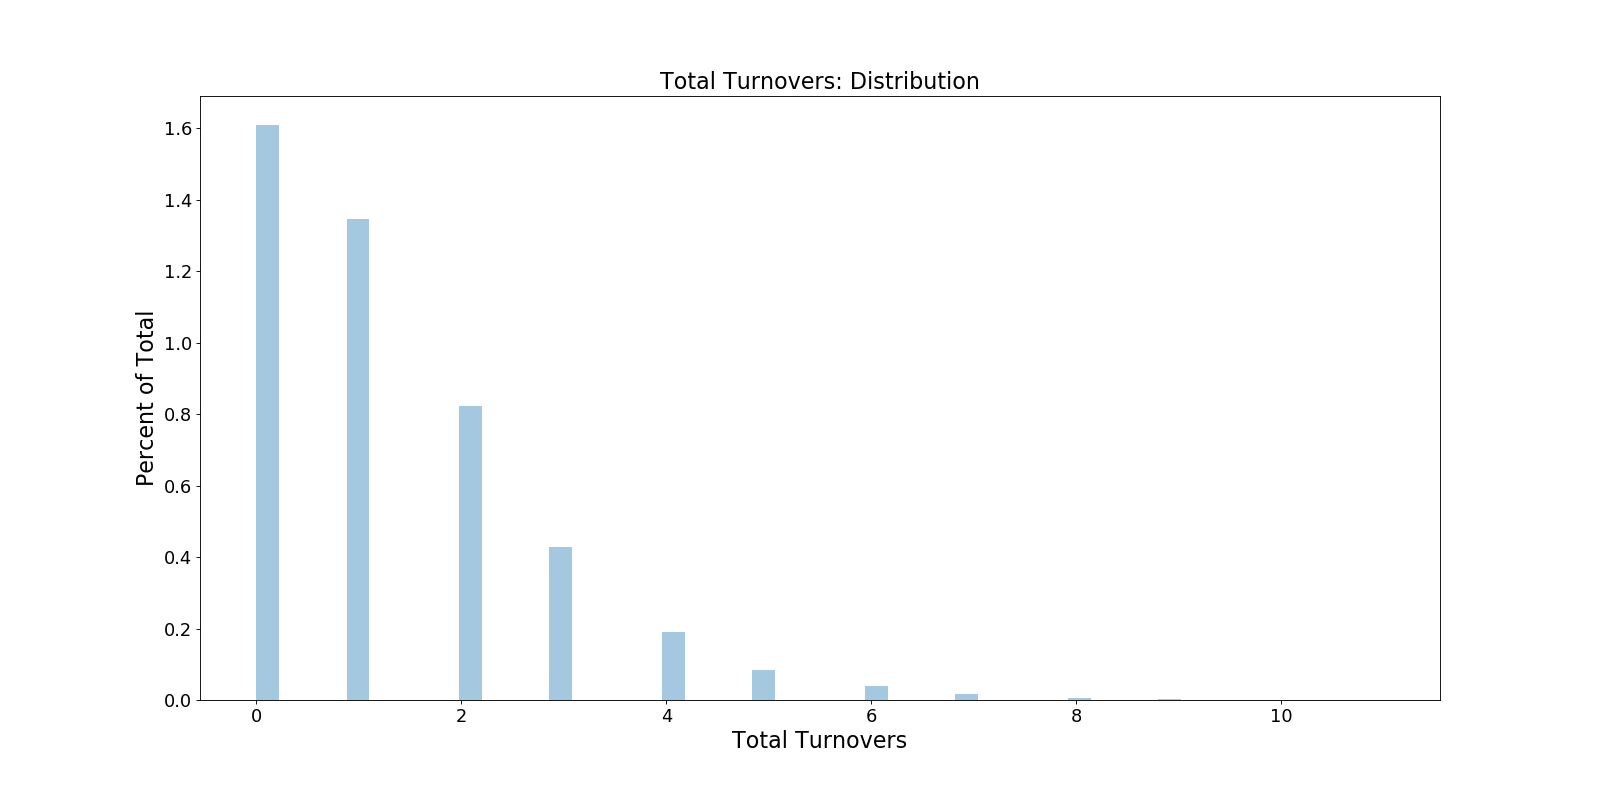
\includegraphics[scale=0.3]{Turnovers_Distribution}\\
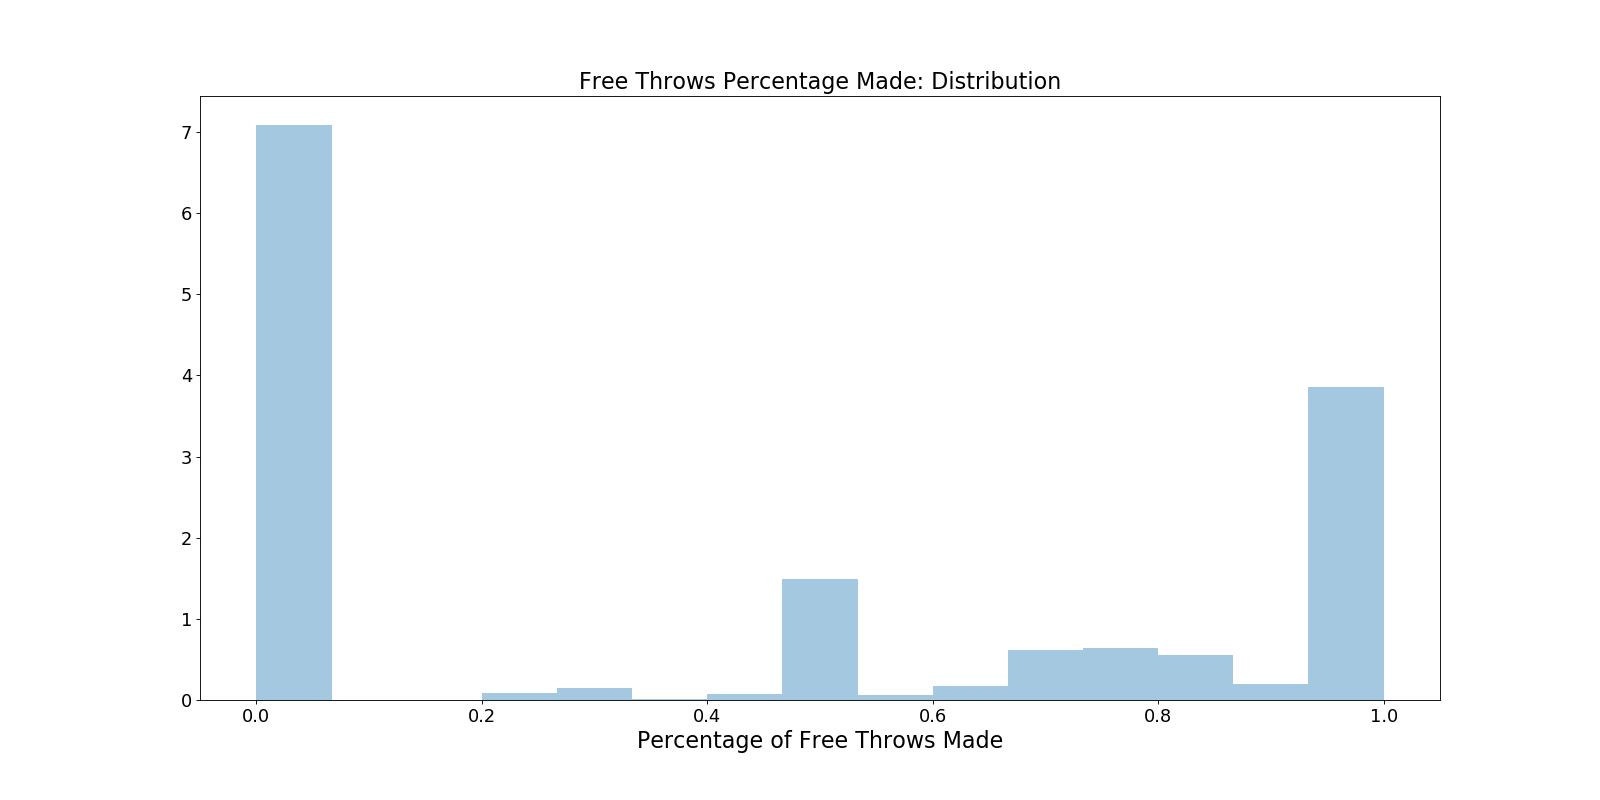
\includegraphics[scale=0.3]{Free_Throw_Percent_Distribution}\\

\section{Game Value Index} \label{game_value_dist}
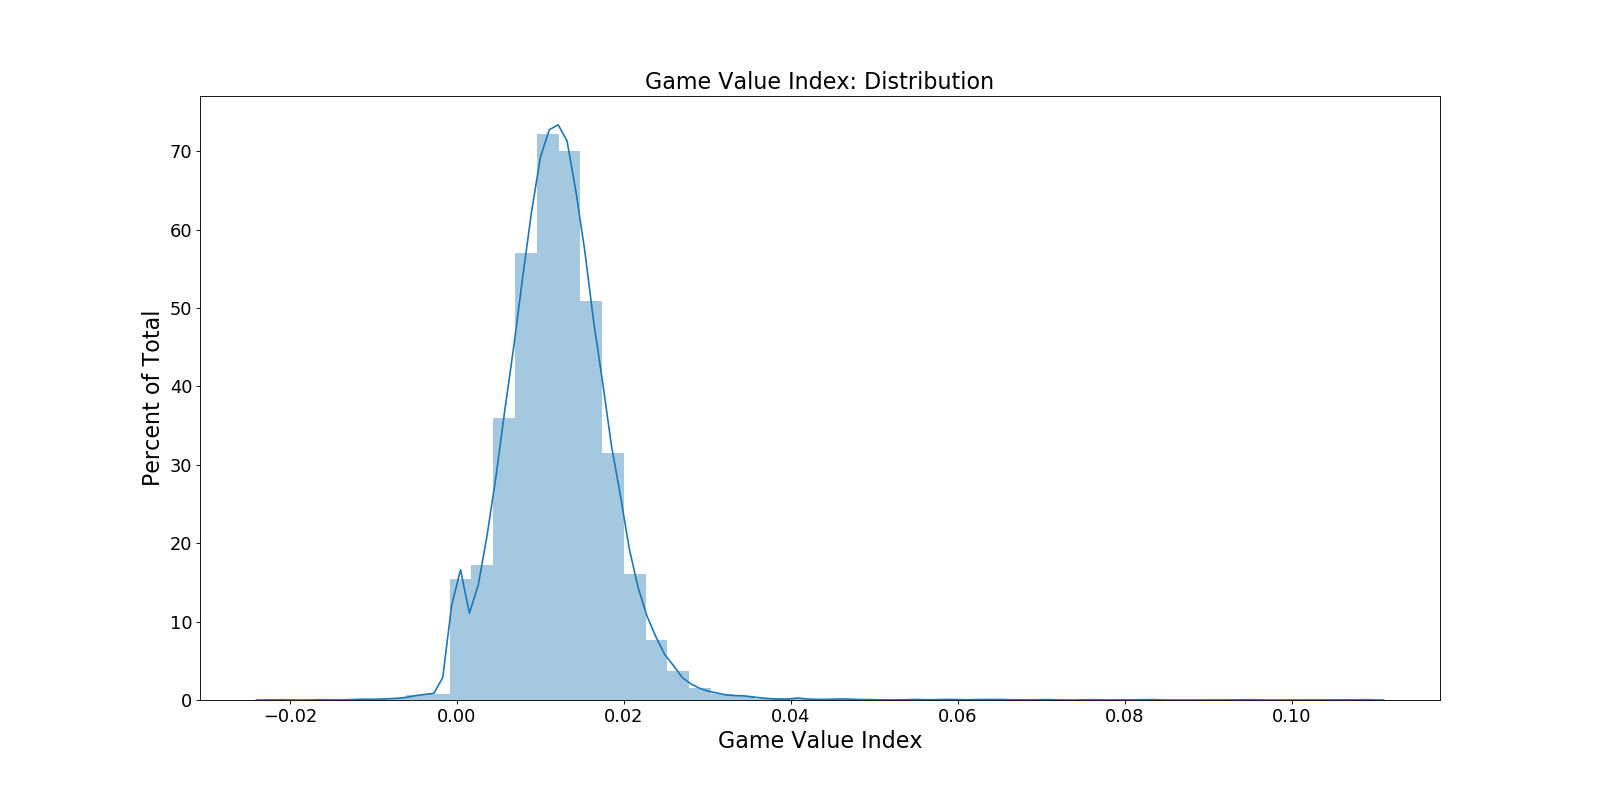
\includegraphics[scale=0.3]{gamevalueIndex}\\

\section{Algorithm in Python} \label{algo}
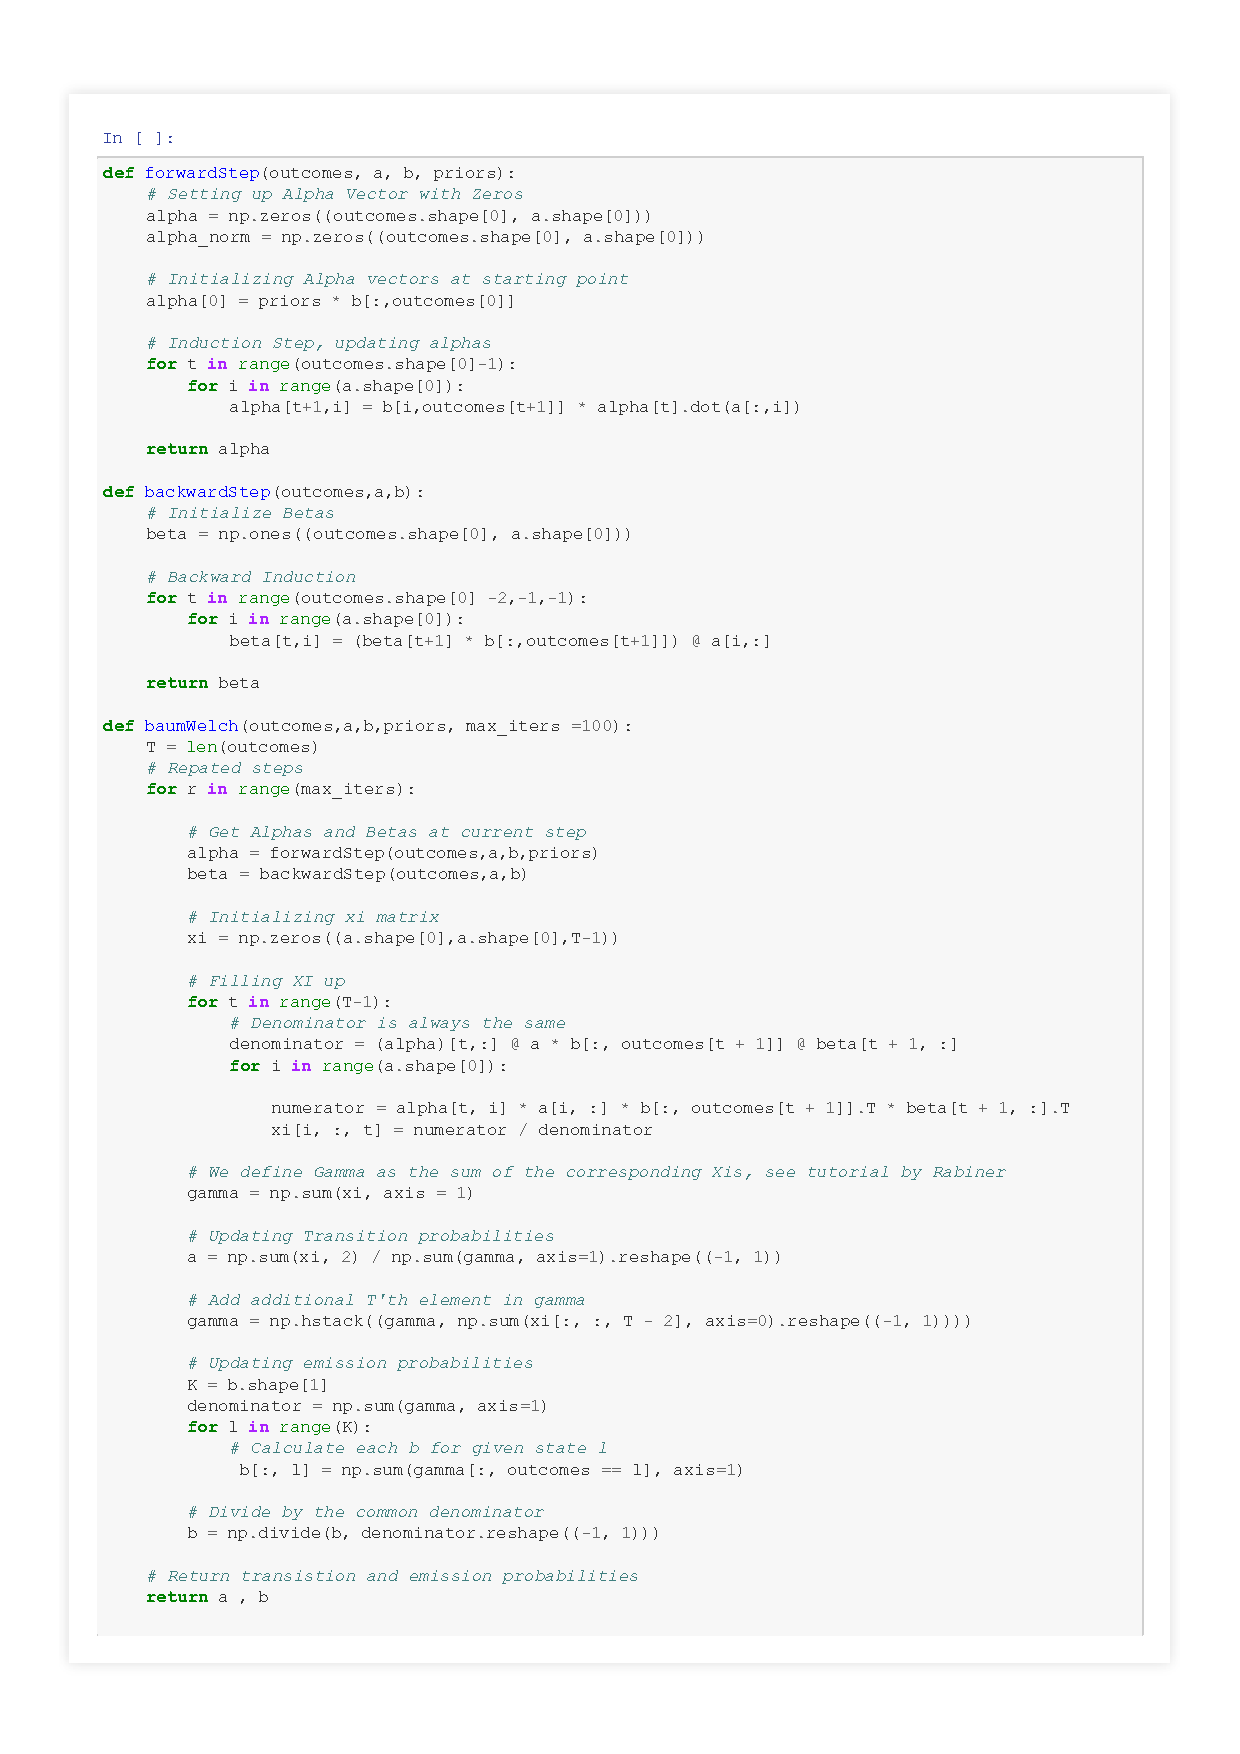
\includepdf[pages=-]{BaumWelch.pdf}
\section{Top Players}\label{top_players}

\begin{tabular}{ |p{3cm}||p{2cm}|p{2cm}|p{2cm}|p{2cm}|  }
	\hline
	\multicolumn{5}{|c|}{Transition matrix of top players in the NBA 2017 - 2018 season} \\
	\hline
	Player Name & Cold Cold & Cold Hot &Hot Cold & Hot Hot\\
	\hline
	Karl-Anthony Towns&   0.112 &	0.888 &	0.389 &	0.611\\
	Anthony Davis&   0.144&	0.856&	0.346&	0.654\\
	LeBron James &0.141&	0.859&	0.345&	0.655\\
	Hassan Whiteside    &	0.070&	0.930&	0.399&	0.601\\
	Joel Embiid&   0.124&	0.876&	0.352&	0.648\\
	DeMarcus Cousins& 0.144&	0.856&	0.345&	0.655\\
	Russell Westbrook& 0.045&	0.955&	0.433&	0.567\\
	Stephen Curry& 0.008&	0.992&	0.354&	0.646\\
	James Harden&  0.011&	0.989&	0.493&	0.507\\
	\hline
\end{tabular}

\begin{tabular}{ |p{3cm}||p{1.5cm}|p{1.5cm}|p{1.5cm}|p{1.5cm}|p{1.5cm}|p{1.5cm}|  }
	\hline
	\multicolumn{7}{|c|}{Emision matrix of top players in the NBA 2017 - 2018 season} \\
	\hline
	Player Name &Bad Cold& Average Cold&	Good Cold&	Bad Hot&	Average Hot&	Good Hot\\
	\hline
	Karl-Anthony Towns&   0.040&	0.455&	0.505&	0&	0.065&	0.935\\
	Anthony Davis&   0&	0.131&	0.869&	0&	0.115&	0.885\\
	LeBron James &0&	0.117&	0.883&	0&	0.107&	0.893\\
	Hassan Whiteside    &0.062&	0.354&	0.584&	0&	0.061&	0.939\\
	Joel Embiid& 0& 0.185&	0.815&	0&	0.015&	0.985\\
	DeMarcus Cousins& 0&	0.117&	0.883&	0&	0.099&	0.901\\
	Russell Westbrook& 0&	0.282&	0.718&	0&	0&	1\\
	Stephen Curry& 0&	0.451&	0.549&	0&	0&	1\\
	James Harden&  0&	0.126&	0.874&	0&	0&	1\\
	\hline
\end{tabular}

\begin{tabular}{ |p{3cm}||p{2cm}|p{2cm}|p{2cm}|p{2cm}|  }
	\hline
	\multicolumn{5}{|c|}{Transition matrix of top players in the NBA 2018 - 2019 season} \\
	\hline
	Player Name & Cold Cold & Cold Hot &Hot Cold & Hot Hot\\
	\hline
	Giannis Antetokounmpo&   0.118 &	0.882 &	0.353 &	0.647\\
	Anthony Davis&   0.129&	0.871&	0.359&	0.641\\
	LeBron James &0.137&	0.863&	0.341&	0.659\\
	Joel Embiid&   0.143&	0.857&	0.356&	0.644\\
	Russell Westbrook& 0.146&	0.854&	0.346&	0.654\\
	Kevin Durant&   0.060&	0.940&	0.440&	0.560\\
	Stephen Curry& 0.000&	1.000&	0.499&	0.501\\
	James Harden&  0.011&	0.989&	0.459&	0.541\\
	\hline
\end{tabular}

\noindent\begin{tabular}{ |p{3cm}||p{1.5cm}|p{1.5cm}|p{1.5cm}|p{1.5cm}|p{1.5cm}|p{1.5cm}|  }
	\hline
	\multicolumn{7}{|c|}{Emision matrix of top players in the NBA 2018 - 2019 season} \\
	\hline
	Player Name &Bad Cold& Average Cold&	Good Cold&	Bad Hot&	Average Hot&	Good Hot\\
	\hline
	Giannis Antetokounmpo&   0&	0.124&	0.876&	0&	0.014&	0.986\\
	Anthony Davis&   0.062&	0.078&	0.861&	0&	0.071&	0.929\\
	LeBron James &0&	0.082&	0.918&	0&	0.075&	0.925\\
	Joel Embiid& 0& 0.171&	0.829&	0&	0.094&	0.906\\
	Russell Westbrook& 0&	0.136&	0.864&	0&	0.098&	0.902\\
	Kevin Durant&   0.046&	0.420&	0.534&	0&	0.039&	0.961\\
	Stephen Curry& 0.050&	0.527&	0.423&	0&	0.061&	0.939\\
	James Harden&  0&	0.184&	0.816&	0&	0&	1\\
	\hline
\end{tabular}


\section{Bad Players} \label{bad_players}
\begin{tabular}{ |p{3cm}||p{2cm}|p{2cm}|p{2cm}|p{2cm}|  }
	\hline
	\multicolumn{5}{|c|}{Transition matrix of bad players in the NBA 2017 - 2018 season} \\
	\hline
	Player Name & Cold Cold & Cold Hot &Hot Cold & Hot Hot\\
	\hline
	Wesley Johnson&   0.799 &	0.201 &	1 &	0\\
	Alex Abrines&   0.574&	0.426&	1&	0\\
	Solomon Hill &0.846&	0.154&	1&	0\\
	Wilson Chandler&   0.641&	0.359&	1&	0\\
	Skal Labissiere& 0.648&	0.352&	0.852&	0.149\\
	\hline
\end{tabular}

\noindent\begin{tabular}{ |p{3cm}||p{1.5cm}|p{1.5cm}|p{1.5cm}|p{1.5cm}|p{1.5cm}|p{1.5cm}|  }
	\hline
	\multicolumn{7}{|c|}{Emision matrix of bad players in the NBA 2017 - 2018 season} \\
	\hline
	Player Name &Bad Cold& Average Cold&	Good Cold&	Bad Hot&	Average Hot&	Good Hot\\
	\hline
	Wesley Johnson&  0.901&	0&	 0.099&	0.002&	0.995&	0.004\\
	Alex Abrines&    1&	    0&    	0&  0.363&	0.318&	0.318\\
	Solomon Hill&    0.899&	0.101&	0&  0.006&	0.821&	0.173\\
	Wilson Chandler& 0.851& 0.149&	0&	0.008&	0.733&	0.260\\
	Skal Labissiere& 0.817&	0.019&	0.164&0.006&0.994&	0\\
	\hline
\end{tabular}


\end{document}